\newpage
\subsection{Finanzierung und wirtschaftliche Machbarkeit}\label{labelWirtMach}
%Gesamtplan 3-5 Jahre

Für die Berechnung unserer Finanzierung und der wirtschaftlichen Machbarkeit werden folgende Annahmen getroffen:

Als einzelne Kostenpositionen erwarten wir folgende Posten:
\begin{itemize}
\item Fixkosten
 \begin{itemize}
\item Serverkosten
\item Lizenzkosten
\item Personalkosten
\item Büromiete
 \end{itemize}
\item variable Kosten
\begin{itemize}
\item Marketingkosten
\item Entwicklungskosten
\item Bürobedarf
\end{itemize}
\end{itemize}

Die Kosten für die Server ergeben sich aus den Betrachtungen im Kapitel \ref{labelTechMach}. Die vermuteten Kosten für das Büro sind dem aktuellen Hamburger Mietspiegel entnommen. Die Personalkosten verteilen sich auf die fünf Mitglieder dieses Unternehmens.

Wie in Kapitel \ref{labelMarktuntersuchung} beschrieben erwarten wir folgende Kunden um Umsätze zu erlösen:
\begin{itemize}
\item Kunde A
\item Kunde B
\item Kunde C
\item Kunde D
\item Kunde E
\end{itemize}

Wir wollen mit unsren Kunden eine langfristige Geschäftsbeziehung eingehen. Wir setzen dabei darauf, dass wir nur einige wenige Kunden benötigen. Durch diese wenigen Kunden können wir aber hohe Umsätze erzielen.
Dabei wollen wir im ersten Quartal 2012 mit Kunde A anfangen und gemeinsam mit dem Kunden die Integration der Zahlungsabwicklung erweitern. Dadurch erhöhen sich die Umsätze in den darauffolgenden Quartalen steig.\\
Ab dem dritten Quartal 2012 gewinnen wir Kunde B und Kunde C als neue Kunden hinzu und im ersten Quartal 2013 zusätzlich Kunde D.\\
Ab dem ersten Quartal 2014 wollen wir in den internationalen Markt expandieren. Dazu wollen wir Kunde E gewinnen.

\subsubsection*{Gewinn und Verlustrechnung}
%24 auf monatlicher Basis, danach jährlich
\begin{figure}[htbp]
	\centering
	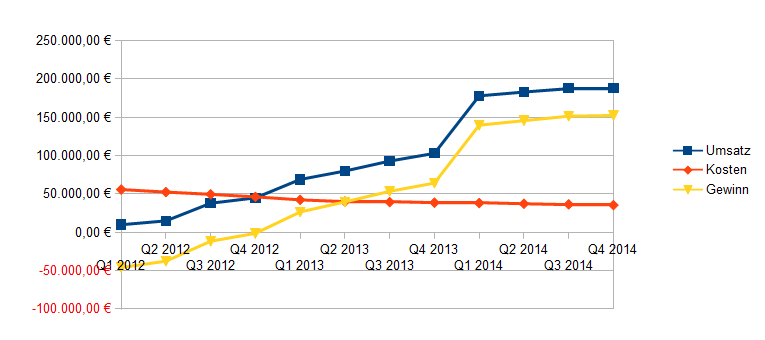
\includegraphics[width=1\textwidth]{geschaeftsplan/GuV.png} 
	\caption{GuV}
	\label{picGuV}
\end{figure}
Für die Berechnung des Gewinns müssen wir berechnen, wie viel ein Spieler im Durchschnitt pro Transaktion ausgibt. Dieser Betrag liegt nach unseren Recherchen bei XX,XX Euro. Dardurch entstehen uns Kosten für die Durchführung der Transaktion. Dieser Betrag liegt im Schnitt bei YY,YY Euro. Diese Kosten, zuzüglich eines Gewinnaufschlags von ZZ,ZZ\% behalten wir für uns ein, der Rest wird an den Kunden weiter gegeben.\\
Dieser Gewinnaufschlag bestimmt unsere Umsätze.

Die erwarteten und aufaddierten Umsätze und Ausgaben sind in der Grafik \ref{picGuV} pro Quartal für die Jahre 2012 bis 2014 dargestellt.

\subsubsection*{Liquiditätsrechnung}
%24 auf monatlicher Basis, danach jährlich
\begin{figure}[htbp]
	\centering
	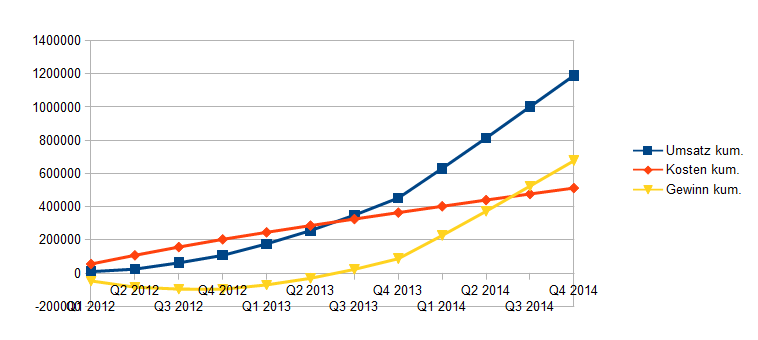
\includegraphics[width=1\textwidth]{geschaeftsplan/GuVkummuliert.png}
	\caption{GuV kumuliert}
	\label{picGuVkum}
\end{figure}

Der Break-Even Punkt wird im ersten Quartal 2013 überschritten. Bis zum vorhergehenden Quartal dahin addieren sich die Verluste auf ca. 90.000,- Euro (s. Grafik \ref{picGuVkum}). Dieser Betrag wird mindestens benötigt, um die zu erwartenden Kosten zu decken.\\
Die Deckung der Kosten wird durch eine Bankfinanzierung geschehen. Dazu nehmen wir einen Kredit in Höhe von 100.000,- Euro auf. Laufzeit 4 Jahre mit einem Zinssatz in Höhe von 5\%. Die monatlichen Tilgungsraten betragen 2.777,78 Euro. Die Kosten sind in den übrigen Berechnungen bereits enthalten.


%\begin{itemize}
%  \item Unsere Finanzierung (Prozentsatz der jeweiligen Transaktionen, Pauschale, Vertrag mit Spielehersteller...)
%  \item Wieviele Nutzer brauchen wir bei welchem Umsatz?
%\end{itemize}
